\documentclass[titlepage]{article}
\usepackage{graphicx}  % 插入图片
\usepackage{amsmath}  % 输入公式
\usepackage{bm}  % 加粗数学符号
\usepackage{listings}  % 插入代码
\usepackage{xcolor}  % 高亮代码
\usepackage{amssymb}  % 空心粗体

% 设置A4纸
\usepackage[a4paper]{geometry} 

\lstset{numbers=left, %设置行号位置
        numberstyle=\tiny, %设置行号大小
        keywordstyle=\color{blue}, %设置关键字颜色
        commentstyle=\color[cmyk]{1,0,1,0}, %设置注释颜色
        frame=single, %设置边框格式
        escapeinside=``, %逃逸字符(1左面的键),用于显示中文
        breaklines, %自动折行
        extendedchars=false, %解决代码跨页时,章节标题,页眉等汉字不显示的问题
        xleftmargin=2em,xrightmargin=2em, aboveskip=1em, %设置边距
        tabsize=4, %设置tab空格数
        showspaces=false %不显示空格
       }

% 文档信息
\title{\textbf{Advanced Control for Robotics: Homework \#1}}
\author{Shang Yangxing}
\date{\today}

\begin{document}

\maketitle

\section{ODE and Its Simulation}

\subsection{Equation of Pendulum Motions}

\begin{figure}[htbp]
    \centering
    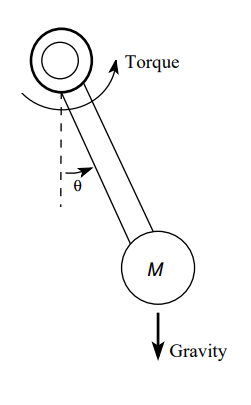
\includegraphics[width=.2\textwidth]{img/pendulum.png}
    \caption{pendulum model}
    \label{fig:pendulum}
\end{figure}

By applying the Newton's law of dynamics, a pendulum with no external force can be formulated as:

\begin{equation}
    ml^2 \ddot{\theta} + ml^2 \alpha \dot{\theta} + mgl \sin{\theta} - T = 0.
\end{equation}

in which,

\quad $m$ is mass of the ball

\quad $l$ is length of the rod

\quad $\alpha$ is the damping constant

\quad $g$ is the gravitational constant

\quad $\theta$ is angle measured between the rod and the vertical axis

\quad $T$ is torque of the joint, which is also the control input $u$

to a system of two first order equation by letting $x_1=\theta$, $x_2=\dot{\theta}$:

\begin{equation}
    \dot{x_1} = x_2, \quad \dot{x_2} = - \frac{g}{l}\sin{x_1} -\alpha x_2 + \frac{T}{ml^2}.
\end{equation}

Written in standard state-space form:

\begin{equation}
    \bm{\dot{x}} = 
    \begin{bmatrix}
        \dot{x_1} \\ \dot{x_2}
    \end{bmatrix}
    =
    \begin{bmatrix}
        x_2 \\ -\frac{g}{l}\sin{x_1} - \alpha x_2
    \end{bmatrix}
    +
    \begin{bmatrix}
        0 \\ \frac{1}{ml^2}
    \end{bmatrix}
    T
    \label{equ:state-space}
\end{equation}

\begin{equation}
    \bm{y} = 
    \begin{bmatrix}
        x_1 \\ x_2
    \end{bmatrix}
    = \bm{x}
\end{equation}

\subsection{Simulation of Pendulum}

When assuming $m=l=1$ with proper unit, equation (\ref{equ:state-space}) can be simplified as:

\begin{equation}
    \begin{bmatrix}
        \dot{x_1} \\ \dot{x_2}
    \end{bmatrix}
    =
    \begin{bmatrix}
        x_2 \\ -g\sin{x_1} - \alpha x_2 + T
    \end{bmatrix}
\end{equation}

according the equation, we code the simulation as following:

\lstinputlisting[language=Python]{simulation_of_pendulum_1_2.py}

and getting the results showed in the Figure \ref{fig:pendulum_sim}

\begin{figure}[htbp]
    \centering
    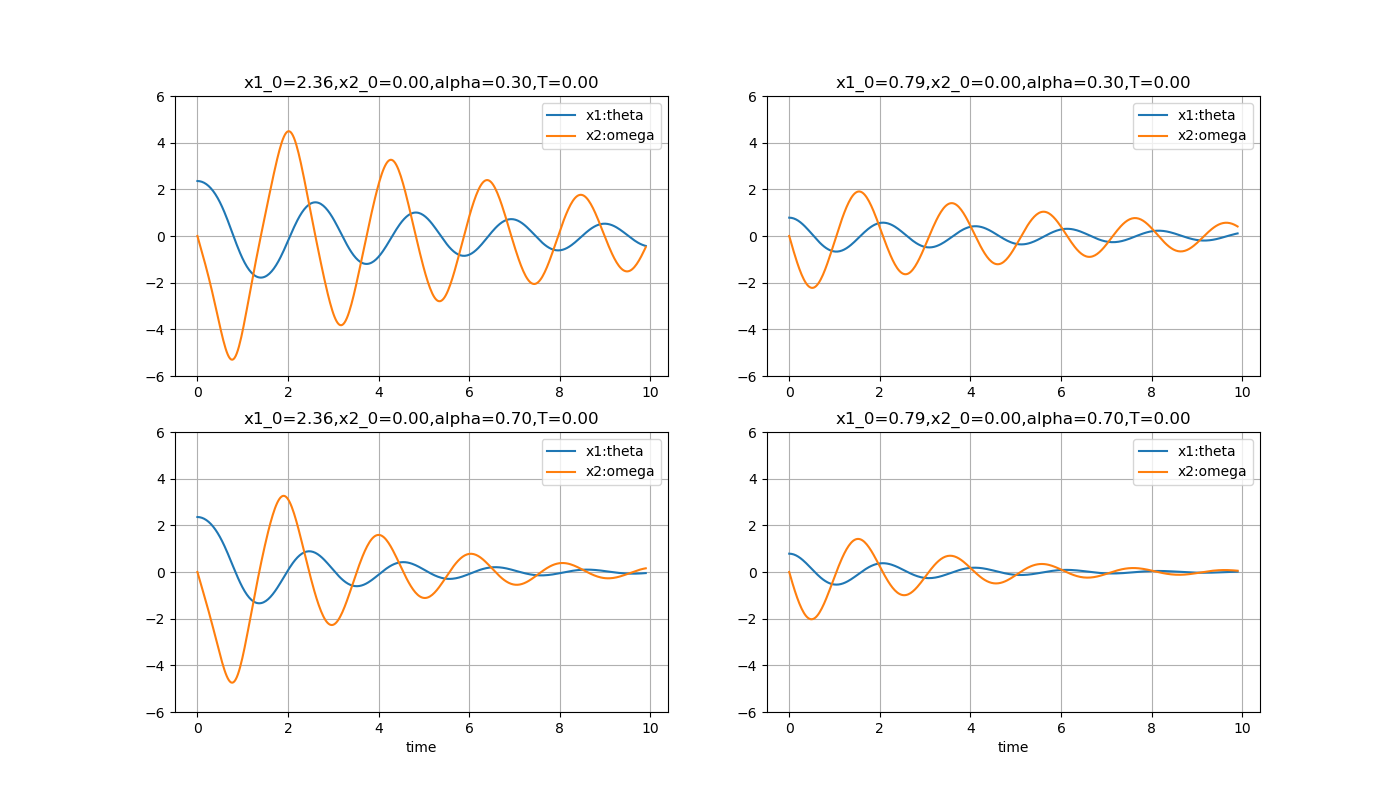
\includegraphics[width=\textwidth]{img/pendulum_sim.png}
    \caption{pendulum simulation output}
    \label{fig:pendulum_sim}
\end{figure}

\section{Matrix calculus}

\subsection{Tutorial}

\begin{equation}
    \frac{\partial}{\partial X}f(X) = 
    \begin{bmatrix}
        \frac{\partial f(X)}{\partial X_{11}} & \cdots & \frac{\partial f(X)}{\partial X_{1m}} \\
        \vdots & \frac{\partial f(X)}{\partial X_{ij}} & \vdots \\
        \frac{\partial f(X)}{\partial X_{n1}} & \cdots & \frac{\partial f(X)}{\partial X_{nm}}
    \end{bmatrix}
    \label{equ:derivativeWRTMat}
\end{equation}

Derivative of scalar function $f(X)$ can be calculated 
by taking derivatives of the scalar function with respect to 
each entry $X_{ij}$ of the matrix $X$ separately, showing 
as above equation (\ref{equ:derivativeWRTMat}). 

Scalar function $f(X)$ project matrix variable 
$X\in\mathbb{R}^{n\times m}$ to a scalar $y\in\mathbb{R}^{1}$,
so its derivative is the partial derivative, except that 
its results are arranged in form of a matrix, who has the same shape as $X$.

For instance, let's say $X=\begin{bmatrix} X_{11}&X_{12}\\X_{21}&X_{22} \end{bmatrix}$,
$f(X)=\begin{bmatrix}1&1\end{bmatrix}\begin{bmatrix}1\\1\end{bmatrix}
\begin{bmatrix} X_{11}&X_{12}\\X_{21}&X_{22} \end{bmatrix}.$
So $y=f(X)=X_{11}+X_{12}+X_{21}+X_{22}.$ And the partial derivative of $f(X)$ is
\begin{equation}
    \frac{\partial}{\partial X}f(X) = 
    \begin{bmatrix} 
        \frac{\partial f(X)}{\partial X_{11}} & \frac{\partial f(X)}{\partial X_{12}} \\ \\
        \frac{\partial f(X)}{\partial X_{21}} & \frac{\partial f(X)}{\partial X_{22}}
     \end{bmatrix}
     =
     \begin{bmatrix} 
        1 & 1 \\
        1 & 1
     \end{bmatrix}
\end{equation}

\subsection{Derivative of Trace}

\begin{equation}
    \begin{aligned}
        \frac{\partial}{\partial X}tr({AX}) &= \frac{\partial}{\partial X} tr(
        \begin{bmatrix}
            A_{11}X_{11} & \cdots & A_{1m}X_{m1} \\
            \vdots & A_{ij}X_{ji} & \vdots \\
            A_{n1}X_{1n} & \cdots & A_{nm}X_{mn}
        \end{bmatrix}) \\
        &= \frac{\partial}{\partial X} 
        (A_{11}X_{11}+\cdots+A_{ij}X_{ji}+\cdots+A_{nm}X_{mn}) \\
        &=
        \begin{bmatrix}
            A_{11} & \cdots & A_{n1} \\
            \vdots & A_{ji} & \vdots \\
            A_{1m} & \cdots & X_{mn}
        \end{bmatrix}=A^T
    \end{aligned}
\end{equation}

in which, $\frac{\partial}{\partial X_{ij}}
(A_{11}X_{11}+\cdots+A_{ij}X_{ji}+\cdots+A_{nm}X_{mn})=A_{ji}$

\subsection{Derivation}

According to \textit{The Matrix Cookbook} equation (81), we have

\begin{equation}
    \frac{\partial x^TQx}{\partial x} = (Q+Q^T)x
    \label{equ:2-3}
\end{equation}

and we can derive that

\begin{equation}
    \frac{\partial tr(xx^T)}{\partial x} = \frac{\partial}{\partial x}(x_1^2+x_2^2+\cdots+x_n^2)=
    \begin{bmatrix}
        2x_1\\2x_2\\\vdots\\2x_n
    \end{bmatrix}
    =2x
\end{equation}

comprehensive above, we get

\begin{equation}
    \begin{aligned}
        \frac{\partial}{\partial x}f(x)
        &= \frac{\partial x^TQx}{\partial x}+\frac{\partial tr(xx^T)}{\partial x} \\
        &= (Q+Q^T)x + 2x
    \end{aligned}
\end{equation}

\section{Inner product}

\subsection{Angle between Two Vectors}

The inner product of two vectors is $<x,y>=\|x\|\|y\|\cos{\theta}$, 
so the angle $\theta$ equal to $\arccos{\frac{<x,y>}{\|x\|\|y\|}}$

\subsection{Compute the Angle}

Using the way to calculate the angle above, we get 

\begin{equation}
    \theta = \arccos{\frac{<A,B>}{\|A\|\|B\|}}
\end{equation}

and we find that

\begin{equation}
    <A,B>=tr(A^TB)=tr(
    \begin{bmatrix}
        -1 & 2 & 1 \\
        -1 & 0 & 1 \\
        -1 & 2 & 1
    \end{bmatrix})
    =0
\end{equation}

so, the angle between A and B is $\frac{\pi}{2}$.

\section{Some linear algebra}

\subsection{Condition}

Take row reducion to $Ax=b$, if any row come up with the situation 
that left-hand side of the equation are zeros, while the right-hand side is not, 
then equation $Ax=b$ has no solution, else it has at least one solution.

\subsection{Compute}

$A$ has two linearly independent columns, so $rank(A)=2$. Knowing $a_3+a_1=a_2$ and $a_4-a_3=a_1$, so we can get $a_3=a_2-a_1$ 
and $a_4=a_1+a_3=a_1+a_2-a_1=a_2$, so

\begin{equation}
    A=[a_1,a_2,a_3,a_4]=[a_1,a_2,a_2-a_1,a_2]
\end{equation}

We can easily find two independent vectors satisfying $Ax=0$

\begin{equation}
    x_1=
    \begin{bmatrix}
        1\\-1\\1\\0
    \end{bmatrix},
    x_2=
    \begin{bmatrix}
        1\\0\\1\\-1
    \end{bmatrix}
\end{equation}

So, $Null(A)=\{x_1,x_2\}$

\section{Gradient Flow}

\subsection{State Space Form}

Let $x_1=\omega, x_2=\dot{\omega}, x=[x_1,x_2]^T$, we get

\begin{equation}
    \dot{x}=
    \begin{bmatrix}
        \dot{x_1}\\\dot{x_2}
    \end{bmatrix}
    =\begin{bmatrix}
        x_2\\-\nabla l(x_1)-Ax_2
    \end{bmatrix}
\end{equation}

\begin{equation}
    y=
    \begin{bmatrix}
        x_1\\x_2
    \end{bmatrix}
\end{equation}

\subsection{Characterize the Equilibrium}

The equilibrium point satisfies $\dot{x}=0$, i.e.

\begin{equation}
    \begin{cases}
        x_2=0\\
        -\nabla l(x_1)-Ax_2=0
    \end{cases}
    \Rightarrow
    \begin{cases}
        \dot{\omega}=0\\
        \nabla l(\omega)=0
    \end{cases}
\end{equation}

\subsection{Simulation}

According to the results in Problem 2.3, i.e. equation (\ref{equ:2-3}), we can derive that

\begin{equation}
    \nabla l(w)=\frac{\partial}{\partial w}(w^TQw+b^Tw)=(Q+Q^T)w+b
\end{equation}

so the system equations can be written as

\begin{equation}
    \begin{bmatrix}
        \dot{x_1}\\\dot{x_2}
    \end{bmatrix}
    =\begin{bmatrix}
        x_2\\-(Q+Q^T)x_1-Ax_2-b
    \end{bmatrix}
\end{equation}

with the system equations, we code the following

\lstinputlisting[language=Python]{simulation_of_accelerated_gradient_5_3.py}

Due to don't knowing the matrix $A$, we assuming that

\begin{equation}
    A=\begin{bmatrix}
        1 & 1 \\ 1 & 1
    \end{bmatrix}
\end{equation}

by switch the cases in the code (line 16),
i.e. change the different matrix $Q$ and $b$,
we get the results showed in Figure \ref{fig:gradient_sim_1} and Figure \ref{fig:gradient_sim_2}

\begin{figure}[htbp]
    \centering
    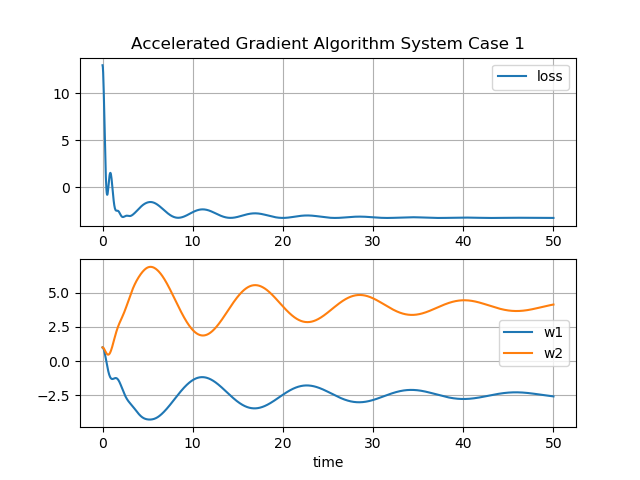
\includegraphics[width=0.8\textwidth]{img/accelerated_gradient_simulation_case_1.png}
    \caption{Accelerated gradient system simulation of case 1}
    \label{fig:gradient_sim_1}
\end{figure}

\begin{figure}[htbp]
    \centering
    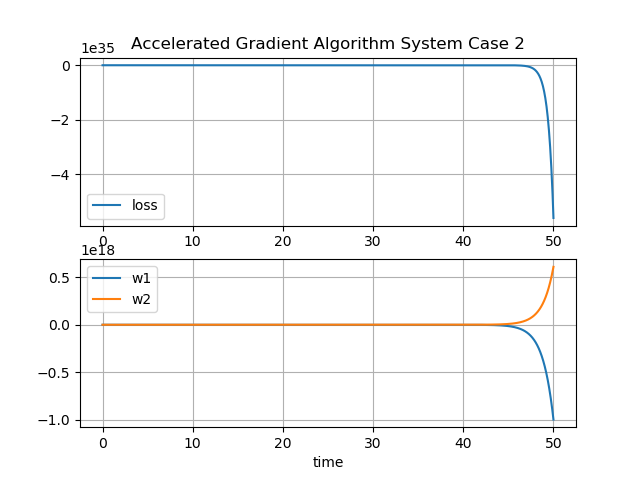
\includegraphics[width=0.8\textwidth]{img/accelerated_gradient_simulation_case_2.png}
    \caption{Accelerated gradient system simulation of case 2}
    \label{fig:gradient_sim_2}
\end{figure}

In the case 1, $Q=\begin{bmatrix} 5&3\\3&2 \end{bmatrix}$,
while in the case 2, $Q=\begin{bmatrix} 1&2\\3&4 \end{bmatrix}$.
Obviously, Figure \ref{fig:gradient_sim_1} shows that the learning in case 1 is successful,
because the loss decreased to a minima and being stable after some epoches.
But case 2 in Figure \ref{fig:gradient_sim_2} is not that successful,
the loss decreased though but not stable, and the loss value is even under $-4\times 10^{35}$,
which is ridiculous.

With more experiments, we find that the value of matrix $A$ could also influence
whether the learning is successful. But it's going to be discussed here.

Also, there is a trick when coding the simulation, specifically,
the args $var\_x$ of the system function $accelerated\_gradient$
should have one dimension, which is decided by the package $scipy.integrate.solve_ivp$.
However, the initial $var\_x$ should be a matrix, so the solution is to pass a
one-dimension array and reshape it inside the function.

Source code can be find here: https://github.com/LoveThinkinghard/Advanced-Control-for-Robotics-Homework

\end{document}